\documentclass[11pt]{article}
\usepackage[ left=2cm, top=3cm, a4paper, text={17cm, 24cm}]{geometry}
\usepackage{graphicx} % Required for inserting images
\usepackage{pdflscape}
\usepackage[T1]{fontenc}
\usepackage{tgschola}
\usepackage[utf8]{inputenc}
\usepackage{hyperref}
\usepackage{float}

\title{Návrh projektu/zadania z predmetu ITU}
\author{Jaroslav Mervart, Veronika Kubová, Pavel Hýža, Šimon Dufek}
\date{7 November 2025}

\begin{document}

\begin{titlepage}
\begin{center}
    \Huge
	\textsc{Vysoké učení technické v~Brně}\\
    \huge
	{\textsc{Fakulta informačních technologií }}\\
	
	\vspace{\stretch{0.382}}
	\LARGE
	User Interface Programming\,--\,Draft\\
	\Huge
    Kimi - \large Digital Pet Webapp\\
	
	\vspace{\stretch{0.618}}
\end{center}
{\large November 7th 2025 \hfill
Veronika Kubová, Šimon Dufek, Pavel Hýža, Jaroslav Mervart}
\end{titlepage}
\newpage

\section{Team}

\begin{itemize}
    \item Leader: Jaroslav Mervart
    \item Members: Veronika Kubová, Šimon Dufek, Pavel Hýža
\end{itemize}

\section{Assignment}
Our general goal is to make a GUI web game application where the user will be taking care of a fictional simulated creature through various game mechanics like feeding, playing mini-games etc.
Through playing various mini-games the user will be able to gain in-game currency which is used to unlock items like better food, cosmetics and upgrades to mini-games.

\begin{itemize}
    \item Target user: Mainly children, teenagers, and young adults; it can be anyone
    \item Use case: Entertainment, pet caring, mini-games
\end{itemize}

\section{Summary of user surveys}
\begin{itemize}
    \item Recreations of old games in the form of mini-games are appreciated. Likewise, good UX design with meaningful actions and controls is valued.
    \item Progression within mini-games is preferable. Mini-games shouldn't be repetitive and should be modifiable. Experienced users should be able to skip easier segments.
    \item An overall goal in a pet-caring game is desirable but can be tricky to come up with due to the nature of games like these.
    \item Cooking does not have to be a boring necessity or just an addition, it can be fun if the player will have to experiment to make different foods.
\end{itemize}

\section{Summary of existing alternatives research}
\begin{itemize}
    \item The key point of a virtual pet is to offer a sense of ownership/companionship. Pou~\ref{source:others/pou}, Tamagotchi and others achieve that.
    
    \item A virtual pet app should have some mini-games where users will be able to gain in-game currency. Pinball, Solitaire, Dinosaur Runner fulfill this purpose well.
    
    \item Food can provide a fun cooking mechanic which can be a mini-game on its own.
    
    \item It is good to have more than care-taking itself and enrich the gameplay with different experiences. But there needs to be a balance between adding everything and keeping it simple.
\end{itemize}


\newpage


    

\section{GUI Draft - Veronika Kubová}
\subsection{User survey}
The selected individual for this interview was a 18 year old grammar school student who played Pou many years ago but stopped.

\textbf{Question 1:} What did you like about games like Pou?

\textbf{Answer 1:} I liked the cosmetics in Pou and how it would react to things. Either looking in different directions or making sounds.

\textbf{Question 2:} What didn't you like in games like Pou?

\textbf{Answer 2:} There was no goal. It was simple but it got repetitive and boring after a certain point.

\textbf{Question 3:} What goal do you think these games could have?

\textbf{Answer 3:} Maybe a certain upgrading thing or unlocking games and have them available later.

\textbf{Question 4:} What did you think of the minigames?

\textbf{Answer 4:} I think in a pet caring game, 2 or 3 minigames are enough. I would like some that are for more than one player but can be played in person rather than online.

\textbf{Question 5:} What did you think of the layout when caring for the pet?

\textbf{Answer 5:} I liked the fridge - you instantly know what foods you have. And the icons were good. The rooms were simple with clear functions but the outside "room" was a bit pointless.

\textbf{Question 6:} Would you play a pet-caring game again? What would it need to have?

\textbf{Answer 6:} Probably not. Maybe if it looked visually appealing or as a platform for simple games like Solitaire, Blockblast or Tetris.

\subsection{Existing solutions analysis}
    \subsubsection{Pou~\ref{source:others/pou}}
    Pou used to be a very popular game in its time and still has many players returning to it due to nostalgia. However, decades later, the game looks very much the same and has not had any major gameplay updates. This beggs the question, what made Pou so great and where is it lacking?

\textbf{Positives}
    \begin{itemize}
        \item Pou isn't solely a pet-caring game and has many minigames that are integrated in the overall gameplay. They are essential for earning in-game currency and subsequently various cosmetincs and foods.
        \item Pou has a few indicators to tell its wellbeing. Namely a health, energy, hunger and hapiness bar. For example, energy can be refilled by letting Pou sleep and closing the game. But if the player doesn't wish to wait, they can use a potion bought with in-game currency to refill it faster.
        \item The character of Pou is the most important part of this game and so he's the central piece of every room he's in, also being a part of every minigame.
    \end{itemize}

\textbf{Negatives}
    \begin{itemize}
        \item Cosmetics are often locked behind high level milestones, making them inaccessible for a very long time and thus demotivating most players.
        \item The layout of the game is made of multiple rooms, each with their own purpose. Moving between them is done via two arrows on the upper side of the screen and the player is unaware which room is on the right or left side.
        \item There are a few less important or unintuitive buttons. One such being a question mark for a hint on how to take care of Pou, or a Pou icon with a number that also leads to settings.
    \end{itemize}

    \subsubsection{Finch~\ref{source:others/finch}}
    Finch is a game mainly focused on mental health and taking care of your "self-care best friend". Instead of staying immersed in the app, it encourages players to interact with the real world but also to stay positive with kind messages. 

    \textbf{Positives}
    \begin{itemize}
        \item  The character Finch isn't limited to body language when it comes to communication. It can also speak through text bubbles, making it more of a friend/child rather than a pet.
        \item The app encourages good habits by offering many features or activities but isn't enforcing them. Leaving it up to the player and whether they have the discipline or motivation to start and continue.
        \item There are daily goals to help build habits with an easy way to check them off.
    \end{itemize}

\textbf{Negatives}
    \begin{itemize}
        \item The app can be a little intimidating at first with many buttons and texts and unclear navigation. The player has to explore everything to get a feel for the layout.
        \item There are also many cosmetics. Some are always accessible, some are time-limited, and some are behind a paywall.
        \item With everything being left up to the player and no clear goal in the game itself, it is easy to stop using.

    \end{itemize}

\subsection{Description of the logical implications of the proposed GUI (individual)}
My part of this project consist of the main screen, which will serve as a starting point of the game, shop for cosmetics and managing energy, food and happiness bars. On the left, there is the initial concept which was then simplified. The most integral parts are the pet itself (which will be able to communicate with the user through text and simple expressions and it will also be moving throughout the room), a sleeping area to recharge energy, a PC that will serve as a menu for certain minigames and to raise happiness and a kitchen for easing hunger and play a cooking minigame.

The bottom part will serve as a status report to check what the creature is feeling and what are its needs currently. The middle is for navigation throughout the room and activities and upper is for settings, shop and achievements.

\begin{figure}[H]
    \centering
    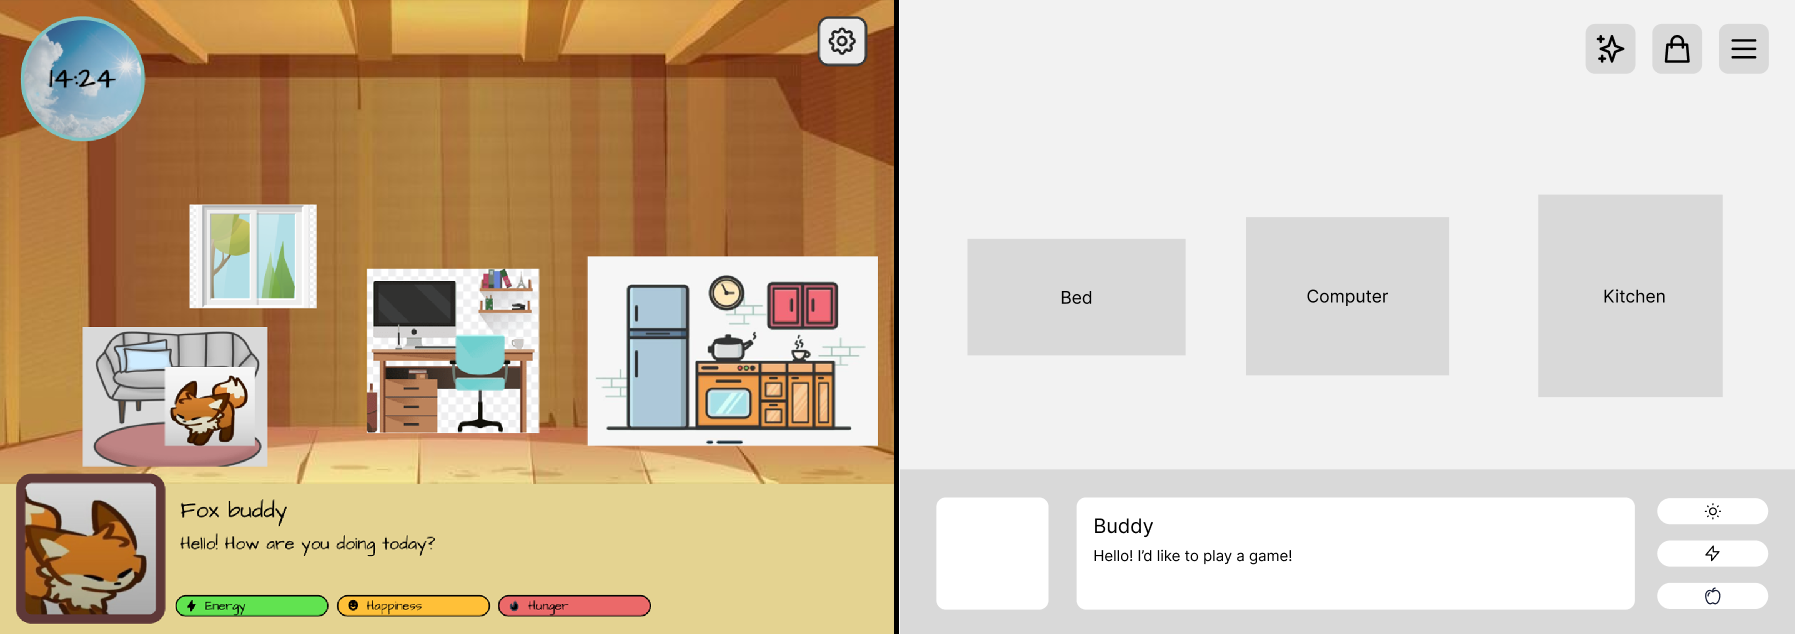
\includegraphics[width=1\linewidth]{pictures/Main screen figma.png}
    \caption{Main menu (concept and layout schowcase)}
    \label{fig:main_menu}
\end{figure}

The kitchen is integral in the hunger mechanic of this game. When the creature is hungry (hunger bar is at 0), it is unable to play games or sleep. However, there will always be free food available that the player can feed to the creature by dragging if from the inventory to the creature standing next to it. There are two ways to obtain food: either by buying it or by cooking it in a minigame.

\begin{figure}[H]
    \centering
    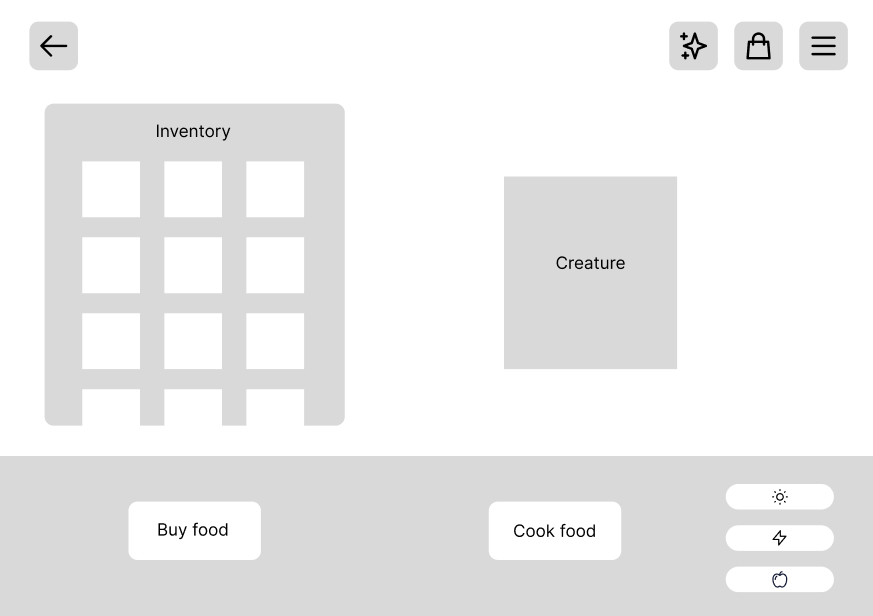
\includegraphics[width=0.5\linewidth]{pictures/Kitchen menu figma.png}
    \caption{Kitchen menu (layout showcase)}
    \label{fig:kitchen_game}
\end{figure}

By clicking on the computer, the player will access a menu from which they can choose which minigame they want to play.

\begin{figure}[H]
    \centering
    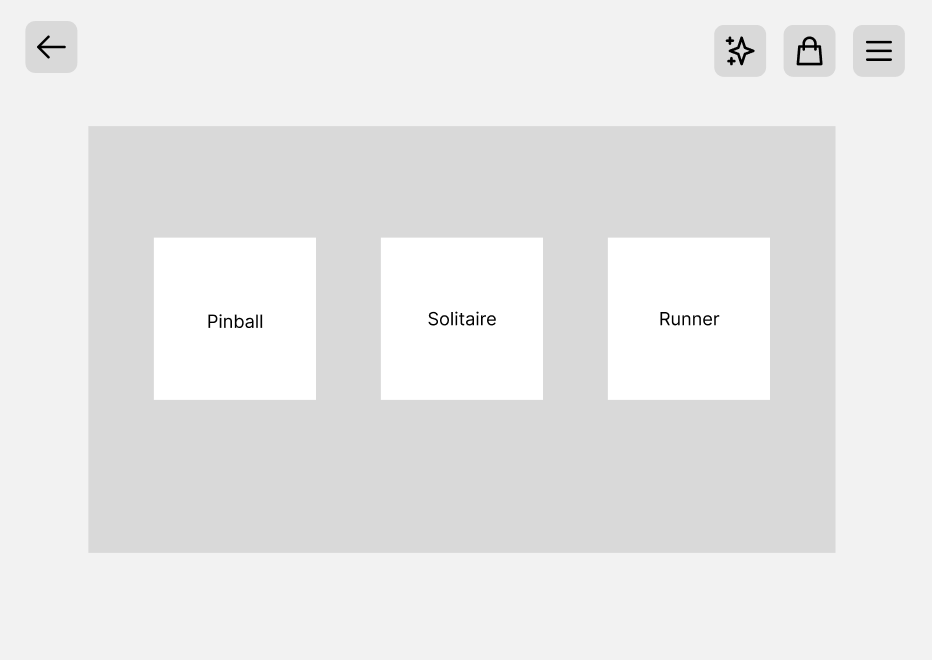
\includegraphics[width=0.5\linewidth]{pictures/PC menu figma.png}
    \caption{PC menu (layout showcase)}
    \label{fig:computer_menu}
\end{figure}

The shop can be accessed from almost anywhere in the game. Though primarily focused on cosmetics, in the future there might be upgrades to certain minigames.

\begin{figure}[H]
    \centering
    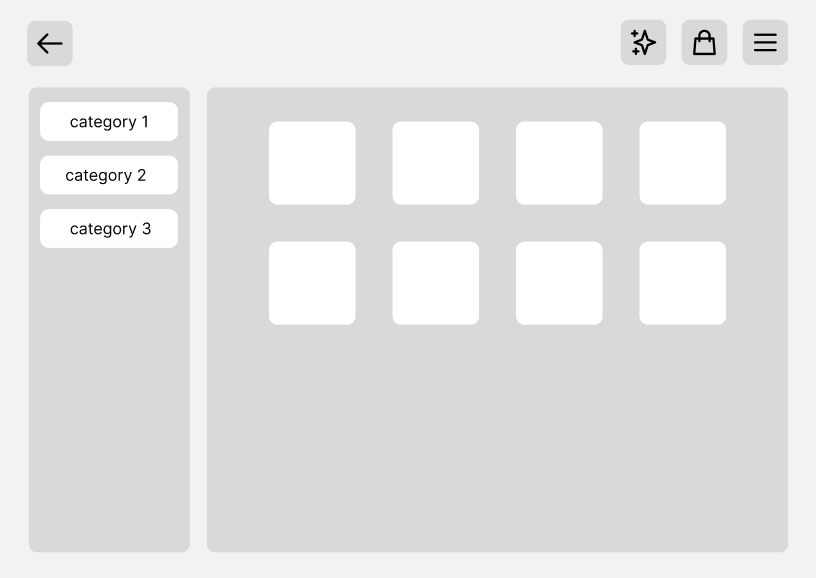
\includegraphics[width=0.5\linewidth]{pictures/Shop figma.png}
    \caption{Shop (layout showcase)}
    \label{fig:shop_layout}
\end{figure}

Below is concept art depicting the creature's appearance.

\begin{figure}[H]
    \centering
    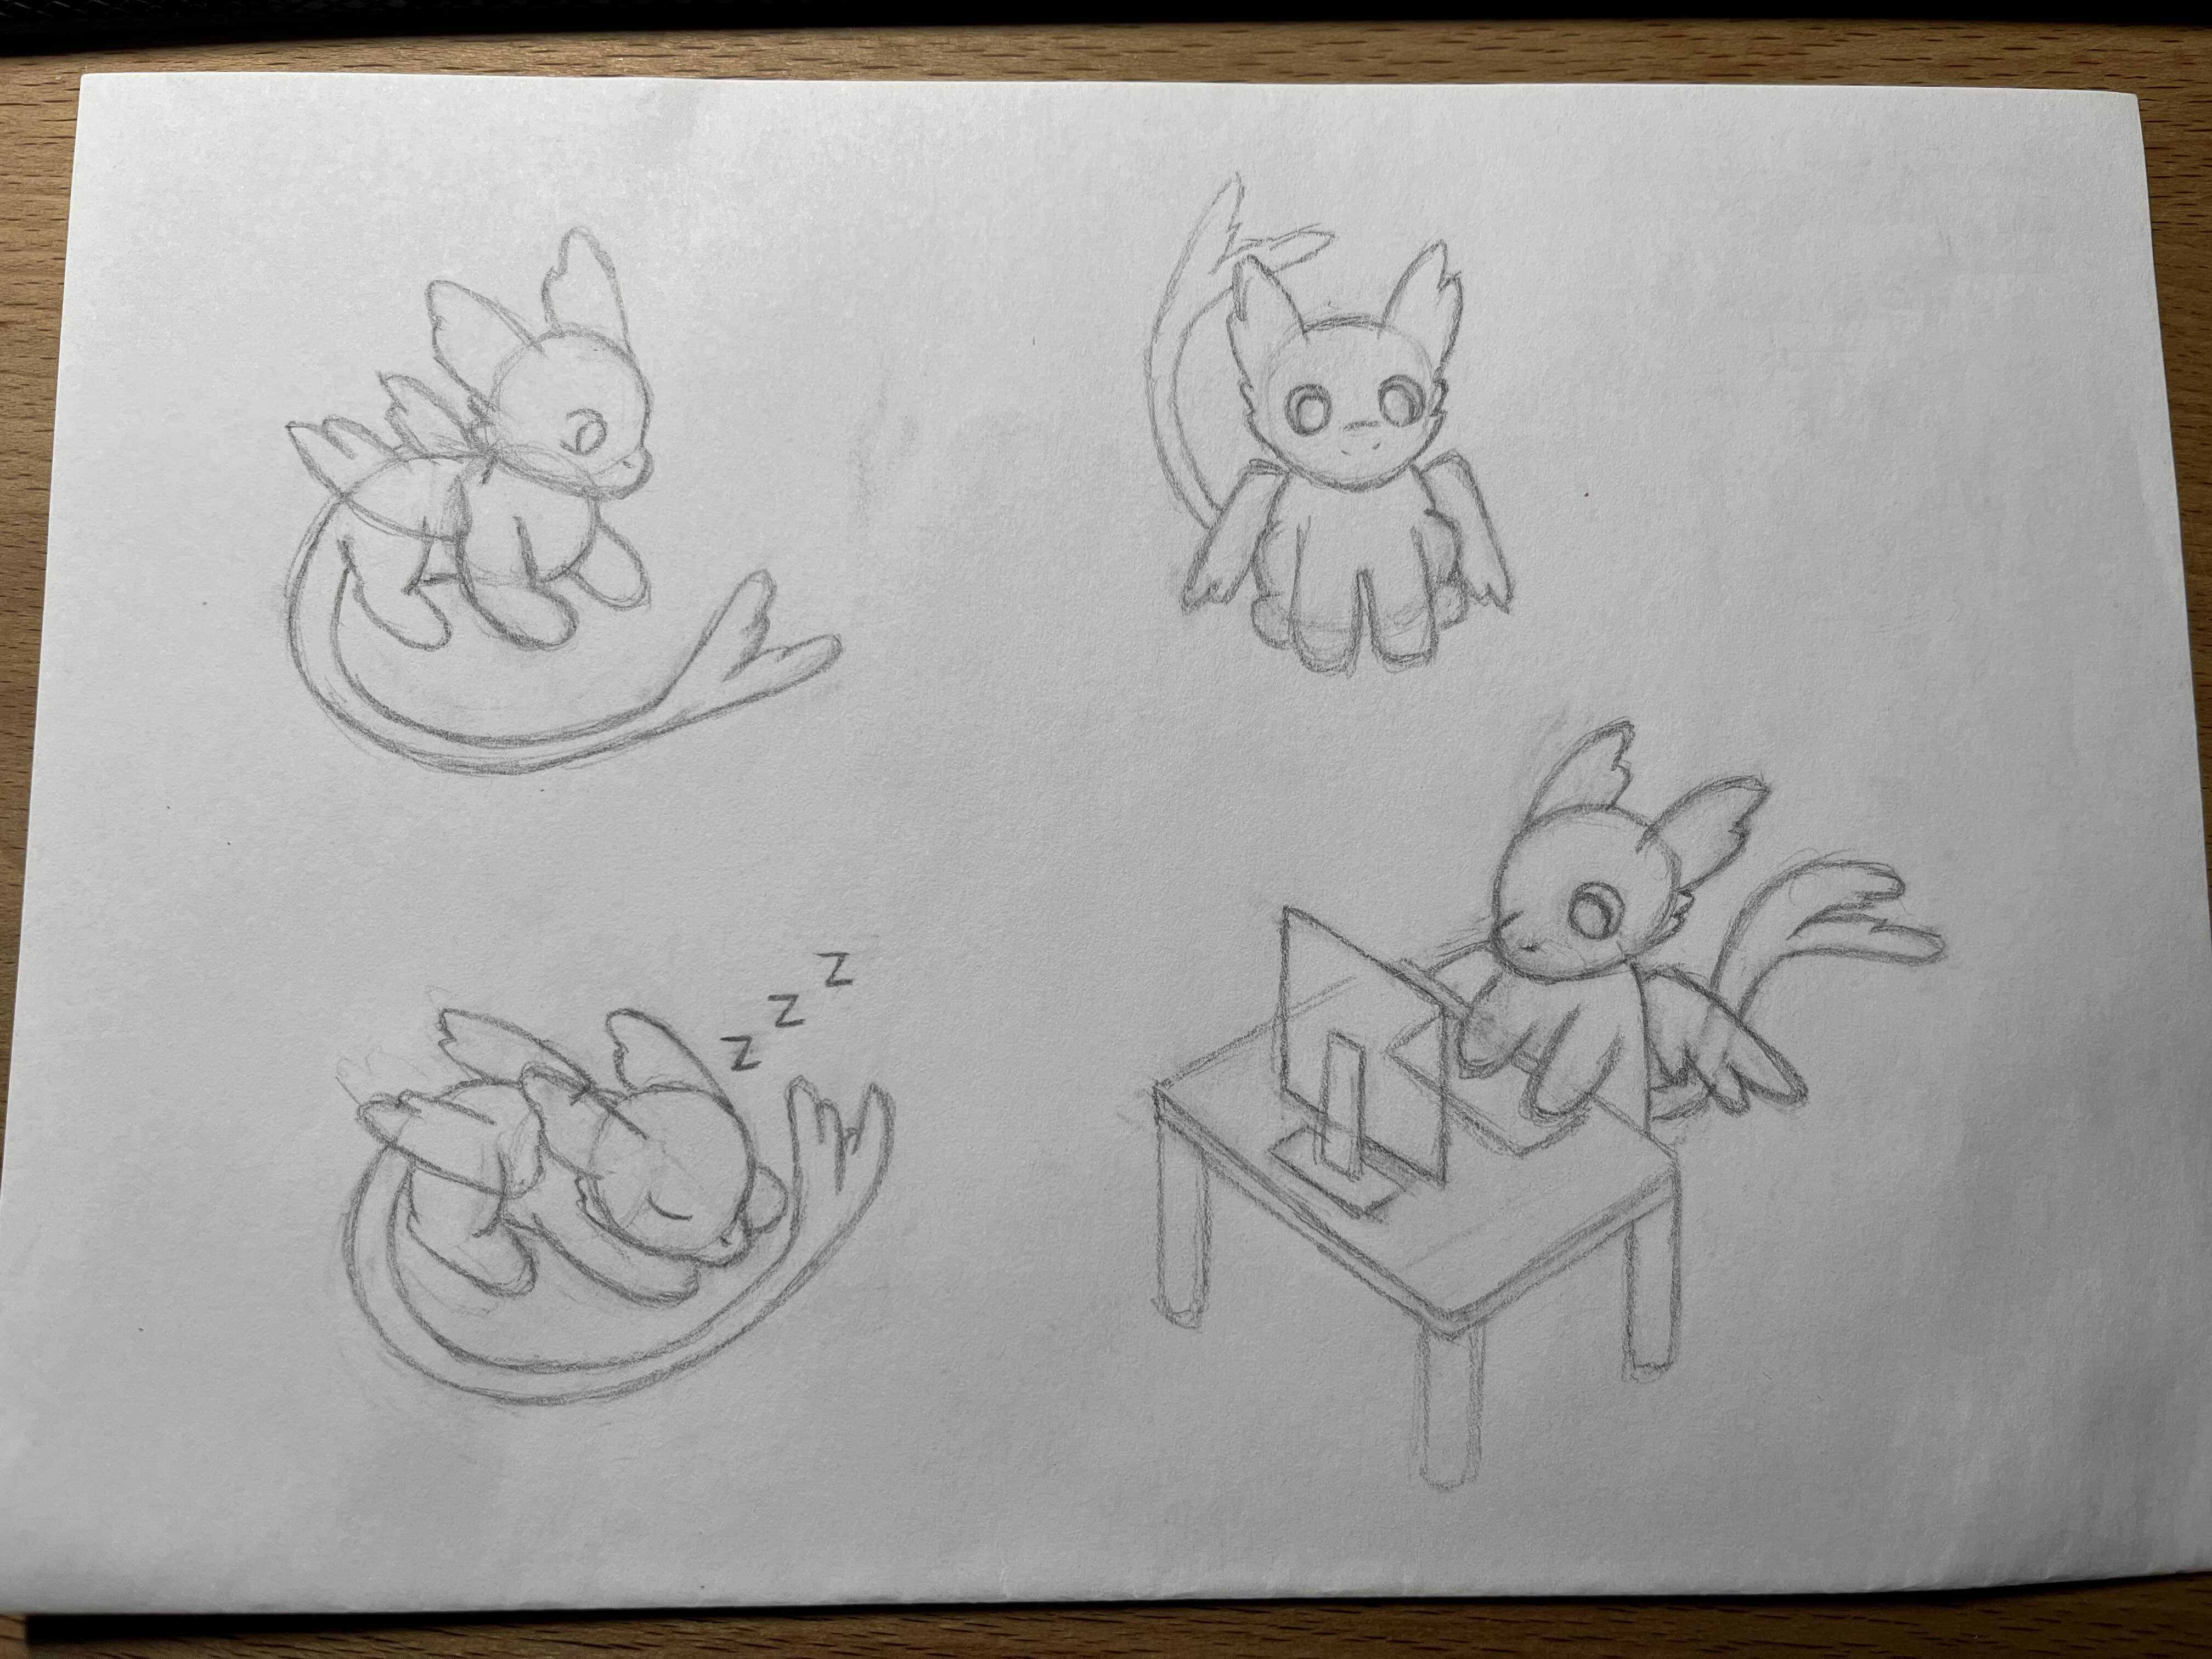
\includegraphics[width=0.5\linewidth]{pictures/Creature (concept).jpg}
    \caption{Creature (concept)}
    \label{fig:creature_art}
\end{figure}

\subsection{How it addresses/reflects user requirements}
By limiting status bars, we also limit the number of areas needed, keeping the design as simple as possible. The main lobby is designed to allow as much interaction between the creature and player as possible while also not blocking the player from wanting to just enjoy the minigames. By adding the shop and achievements, the player has something to work towards, giving them a simple goal. The final impression of the game will partially depend on the chosen artistic style and color scheme.
\newpage




\section{GUI Draft - Šimon Dufek}
\subsection{User survey}
I conducted my survey with a friend from school. We both played Legend of Zelda: Breath of the Wild.

    \textbf{Question 1:} How did you like to cook in Zelda compared to other games?

    \textbf{Answer 1:} I really liked it. It was not just an addition, it had a real effect on the game, it boosted health, stamina, and endurance. Also, it felt audibly and visually pleasing

    \textbf{Question 2:} How did you enjoy experimenting with different ingredients while cooking?

    \textbf{Answer 2:} I spent a lot of time trying different combinations of ingredients and really enjoyed it. If you got the ingredients right you made something nice, if not you made something disgusting, which was also pretty fun.

    \textbf{Question 3:} Was there something that you missed while cooking or something you would like to have been added there?
    
    \textbf{Answer 3:} I might've added something like a recipe book, not to give away the recipes away, but to store the already discovered ones. Sometimes it was quite frustrating when I forgot the recipes I already once discovered and messed it up. It might also be good if there would be more cooking equipment to speed things up.

\subsection{Existing solutions survey}

\subsubsection{Tamaweb~\ref{source:others/tamaweb}}
This game is a recreation of classical Tamagotchi~\ref{source:others/tamagotchi} handheld game. While it tries to preserve the original aspect of the classical game, the UX is lacking, despite it being the point. Most of the screen is blank and unappealing. We should try to use as much of the screen as we can.

\textbf{Positives}
\begin{itemize}
    \item Emotional attachment. There is a connection between the player and the creature, the player has to feed and clean it, and play games to keep it happy.
    \item Cycle of care and rewards. Very clear basic gameplay loop, take care, creature is happy, you get bonuses or mini-games.
    \item Connection of multiple systems into one. The creature was a central element of mini-games, progression points or cosmetics.
\end{itemize}
\textbf{Negatives}
\begin{itemize}
    \item Low interactivity. Very few buttons to press.
    \item Static content. No expansion or evolution, the creature wasn't aging or growing.
    \item Nothing social. The creatures couldn't interact between each other, no sharing, meetings or competitions.
\end{itemize}

\subsubsection{The Legend of Zelda: Breath of the Wild~\ref{source:others/zelda}}
One of the side gameplay mechanics in The Legend of Zelda: Breath of the Wild~\ref{source:others/zelda} is cooking. Users can prepare different meals and experiment, with the possibility of creating \emph{dubious} food (which is mostly waste of ingredients) . While some players rarely use this feature, many enjoy going in blind or simply appreciate the act of cooking itself. Since the cooking process is often soothing, our players might enjoy a similar feature as well.

\newpage
\textbf{Positives}
\begin{itemize}
    \item Experimentation. The player throws different resources into the cauldron and discovers recipes on their own.
    \item Clear reward. Each food has a direct effect on gameplay like giving health, increasing endurance or giving other buffs.
    \item Aesthetic. Short animation and a good sound for success and a better sound for a great success.
\end{itemize}

\textbf{Negatives}
\begin{itemize}
    \item Confusing over time. Once the player has a lot of resources, it is easy to forget what works with what.
    \item Limited to single-player. Cooking doesn't effect the larger world, there is no recipe sharing between players or something like "food of the week".
    \item Repetitive. After a few dozen recipes it becomes just drag and drop, there is no timing, managing heat or other mechanics.
\end{itemize}

\subsection{Description of the proposed GUI}
My proposed section focuses purely on the cooking mini-game. It features the selection of ingredients from a fridge overlay and the ability to keep notes at the top of the screen. Finally, the player can cook the prepared meal — an action that results in either a successful dish with various properties (such as bonuses to other mini-games or status improvements) or negative effects if the recipe is poor. Naturally, the system will need to update itself based on data stored on the server, such as fridge contents (inventory), discovered recipes, and the time the meal has been cooking.

\begin{figure}[H]
    \centering
    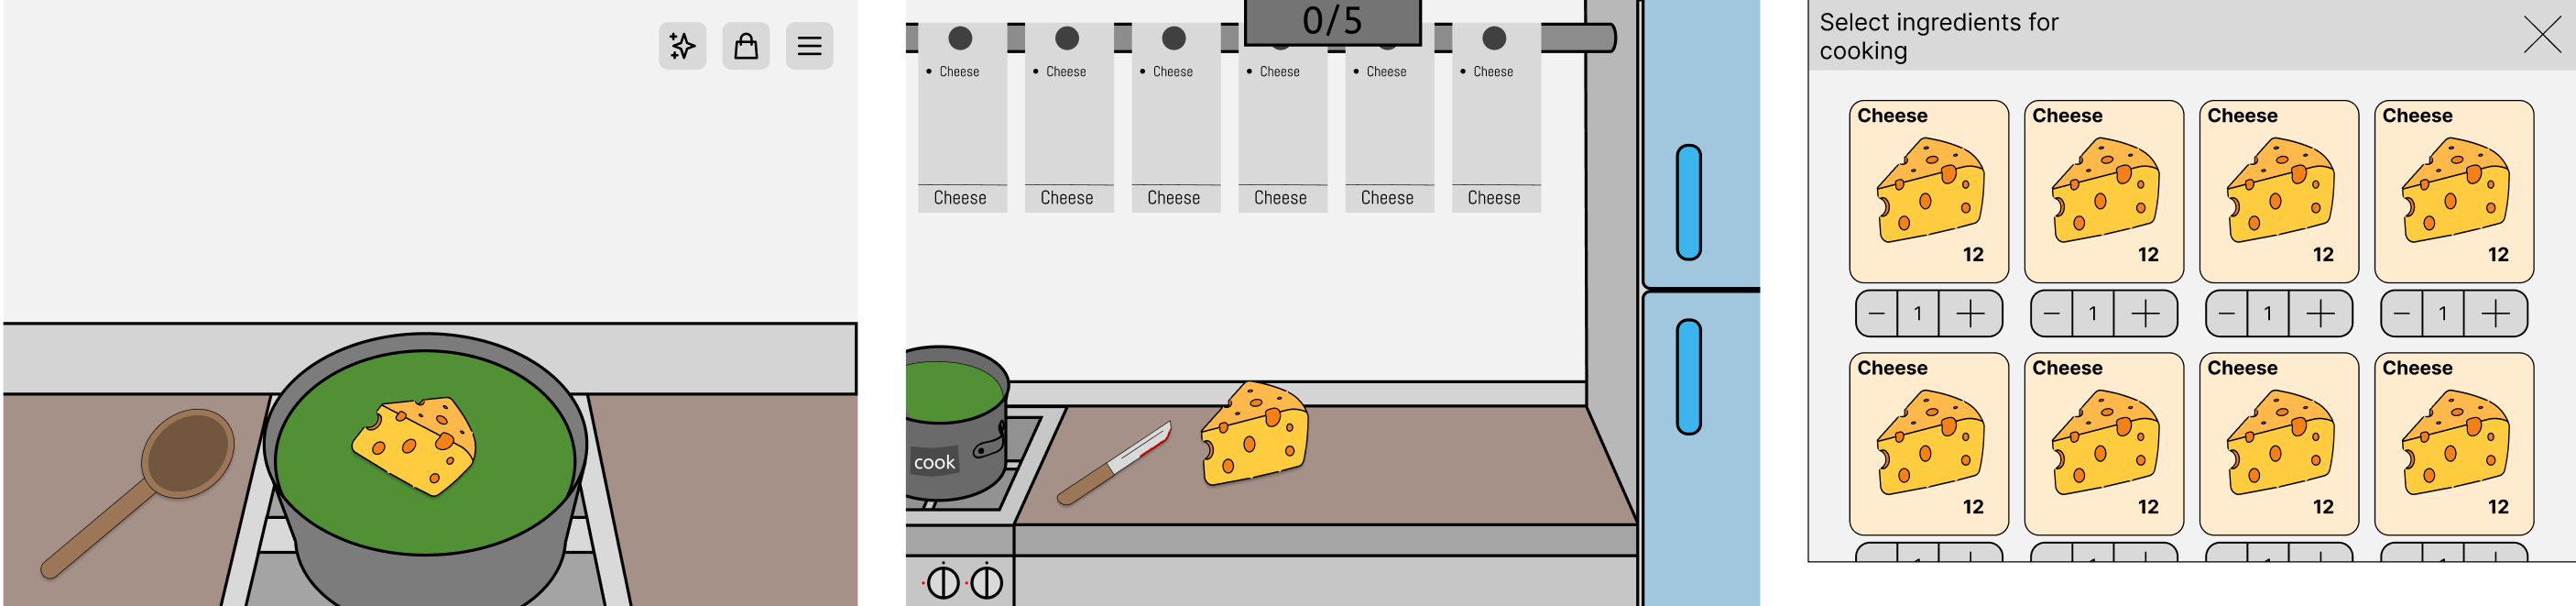
\includegraphics[width=1\linewidth]{pictures/kitchen.png}
    \caption{Kitchen -- cooking process}
    \label{fig:kitchen_action}
\end{figure}

\subsection{How it addresses/reflects user requirements}
The kitchen environment provides the ability to make experimental cooking to give a discovery experience to the player before they feed their pet. If they succeed in cooking they should get a sense of accomplishment. By cooking process not succeeding, user should be motivated to experiment further. We will discuss the possibility of book with discovered recipes. It is still kept simplistic enough for the user to not get lost while having more than enough options to experiment freely.  
\newpage


\section{GUI Draft - Pavel Hýža}
\subsection{User survey}
   The selected individual for this survey is a 22 year old university student who played games like Pou, including it's many mini-games. The selected user's needs of the proposed application are to be entertained as much as possible while recognizing aspects of the games like Pou, which the user did not like while playing them.

    \textbf{Question 1:} When you played Pou, what was the most fun for you about it? Why do you think you played it in the first place?

    \textbf{Answer 1:} It was really fun watching Pou grow and change based on how I was taking care of him. I really thought of him as real person. I liked the sense of progress through the various unlocks of the game.

    \textbf{Question 2:} Was there something that you didn't like about Pou in general, was there something you'd like changed, removed or added?

    \textbf{Answer 2:} I guess it started to feel repetitive, the mini-games were still the same and got boring quite quickly. I also missed a bigger goal or a motivation, getting more money felt pointless at a certain point. I would definitely like more interactions with Pou, it would make it feel more alive.

    \textbf{Question 3:} What did you NOT like about Pou's mini-games? Was there something you would've liked to be changed?
    
    \textbf{Answer 3:} When I got better at some of the mini-games, it got really annoying to have to start over again every time I failed because I'd have to go through the initial slower part of it every time to get to where I was last time.
    
    \textbf{Question 4:} How did you like the way the game handled status bars like health and food? Did you feel like this mechanic was fun for you, or did you feel that it only annoyed you, or something in between?
    
    \textbf{Answer 4:} I felt that the status bar mechanics were OK, they weren't annoying, but not very interesting themselves, I guess you could make them better.

    \textbf{Question 5:} How did you feel in general when playing the game? What feeling did it evoke? Did you mainly want to progress or just relax?

    \textbf{Answer 5:} It was mainly a simple relaxing game. I could turn it on and escape from real life for a few minutes, feed Pou and play a short game while not having to think much about anything.

\subsection{Existing solutions survey}
    \subsubsection{Space Cadet Pinball}
    This is an old Pinball game that ran on Windows XP. The player has to launch a ball into the playing area and then keep it there using controllable elements on the game table to keep in the play for as long as possible and accumulate as much score as they can. I'd like to implement my own version of Pinball as a mini-game in the final application, hence why this is relevant.

    \begin{figure}[!ht]
        \centering
        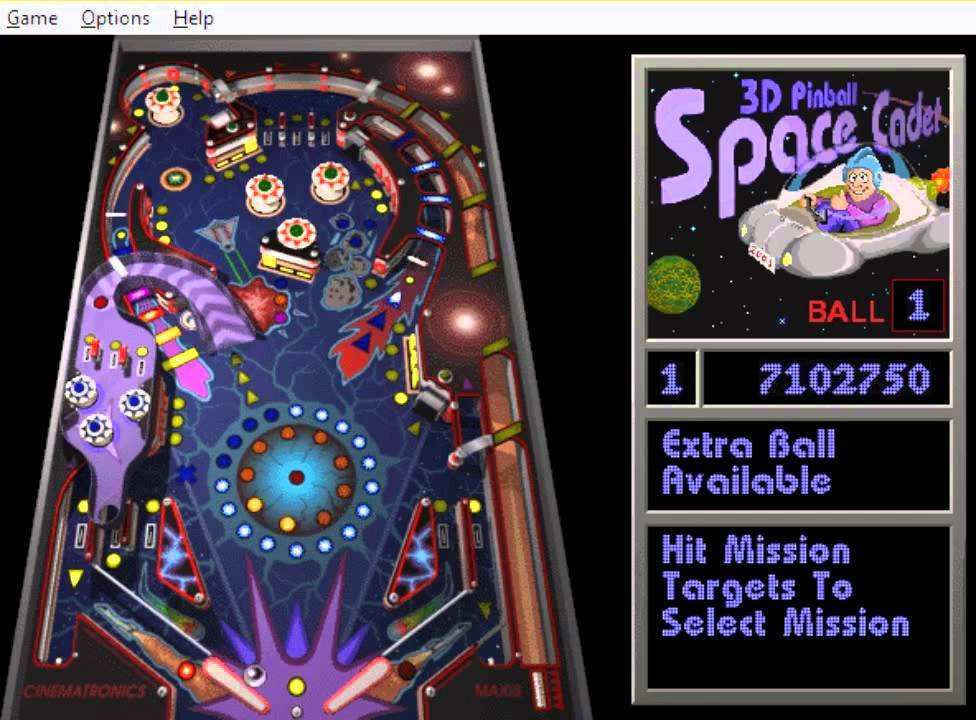
\includegraphics[width=0.75\linewidth]{pictures/Space Cadet.jpg}
        \caption{Space Cadet}
        \label{fig:space_cadet}
    \end{figure}

    \textbf{Positives}
    \begin{itemize}
        \item Missions and rank progression. The game isn't only about holding the ball, but there are special quests and ranks to progress through which also give more rewards.
        \item Audio/visual spectacle. Arrows, lights and sounds give great navigation where to aim and what just activated. The game feels very reactive and alive because of this.
        \item Quick rewarding. Multipliers are gained quickly, there are combo bonuses, ball saving, extra balls. Every good hit is very rewarding and motivate the player to shoot just one more time.
    \end{itemize}

    \textbf{Negatives}
    \begin{itemize}
        \item Outdated technology. The physics engine and camera are very out of date. Flipper reaction time can sometimes be sluggish, and general ball reactiveness can feel weird due to low framerate.
        \item Single run only. There is nothing outside the game itself, no daily quests, seasonals or leaderboards with other players.
        \item Static. There is just one version of the game table, no game modifiers, no way to change the table layout, no cosmetics.
    \end{itemize}

    Full Tilt! Pinball~\ref{source:others/pinball}

    \subsubsection{Dinosaur Game}
    This is a game where a dinosaur character continuously runs forwards and the player has to avoid obstacles in its way by jumping above them or ducking under them. This is the game that is available in Google Chrome whenever the user has no internet access. I'd like to implement a mini-game of similar style, hence the relevance.

    \begin{figure}[!ht]
        \centering
        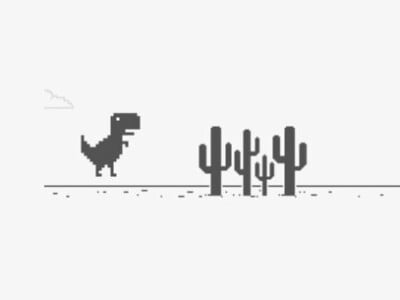
\includegraphics[width=0.75\linewidth]{pictures/Dinosaur Game.jpg}
        \caption{Dinosaur Game}
        \label{fig:dino_game}
    \end{figure}

    \textbf{Positives}
    \begin{itemize}
        \item Very simple. Instant start, intuitive controls, no menu or tutorials, straight gameplay. Good for a quick short game session.
        \item Flow and difficulty scaling. Tempo of the game increases over time, the player has to react faster and better. New types of obstacles appear, day and night changes.
        \item Minimalistic graphics. Simple pixel art, very easy to read, no visual clutter. Works on all devices.
    \end{itemize}

    \textbf{Negatives}
    \begin{itemize}
        \item Single run only. There are no achievements, no purchasable gadgets to get further in the game for in-game money. Everything except the highest achieved score resets when dying in-game.
        \item Limited variety of content. After a few minutes you've seen everything the game has to offer. The same obstacles repeat over and over again. You're still looking at the same cactus and bird.
        \item No customisation. The dinosaur is very simple and you can't change its appearance. Also no score sharing in leaderboards or with friends.
    \end{itemize}
    
    Dinosaur Game~\ref{source:others/dinogame}
    

\subsection{Description of the proposed GUI}
My proposed GUI will consist mainly of 2 mini-games inside the main application. The first mini-game will be a pinball variation, the second mini-game will be a dinosaur runner game variation. Both games will be very simple in their basic state. The user is expected to try out these games and get a small amount of money for the main application shop by playing. Both games will also have extensions and modifications obtainable in the main application shop. These extensions will aim to modify the games to have more gameplay variety, and offer more challenging experience for players who got better at playing them. Both games will also have a scoring mechanic.

The following screenshots showcase what a basic sketch of the mini-games looks like. The text fields in the pictures are only there to illustrate how extensions could look like in the final application.

\begin{figure}[!ht]
    \centering
    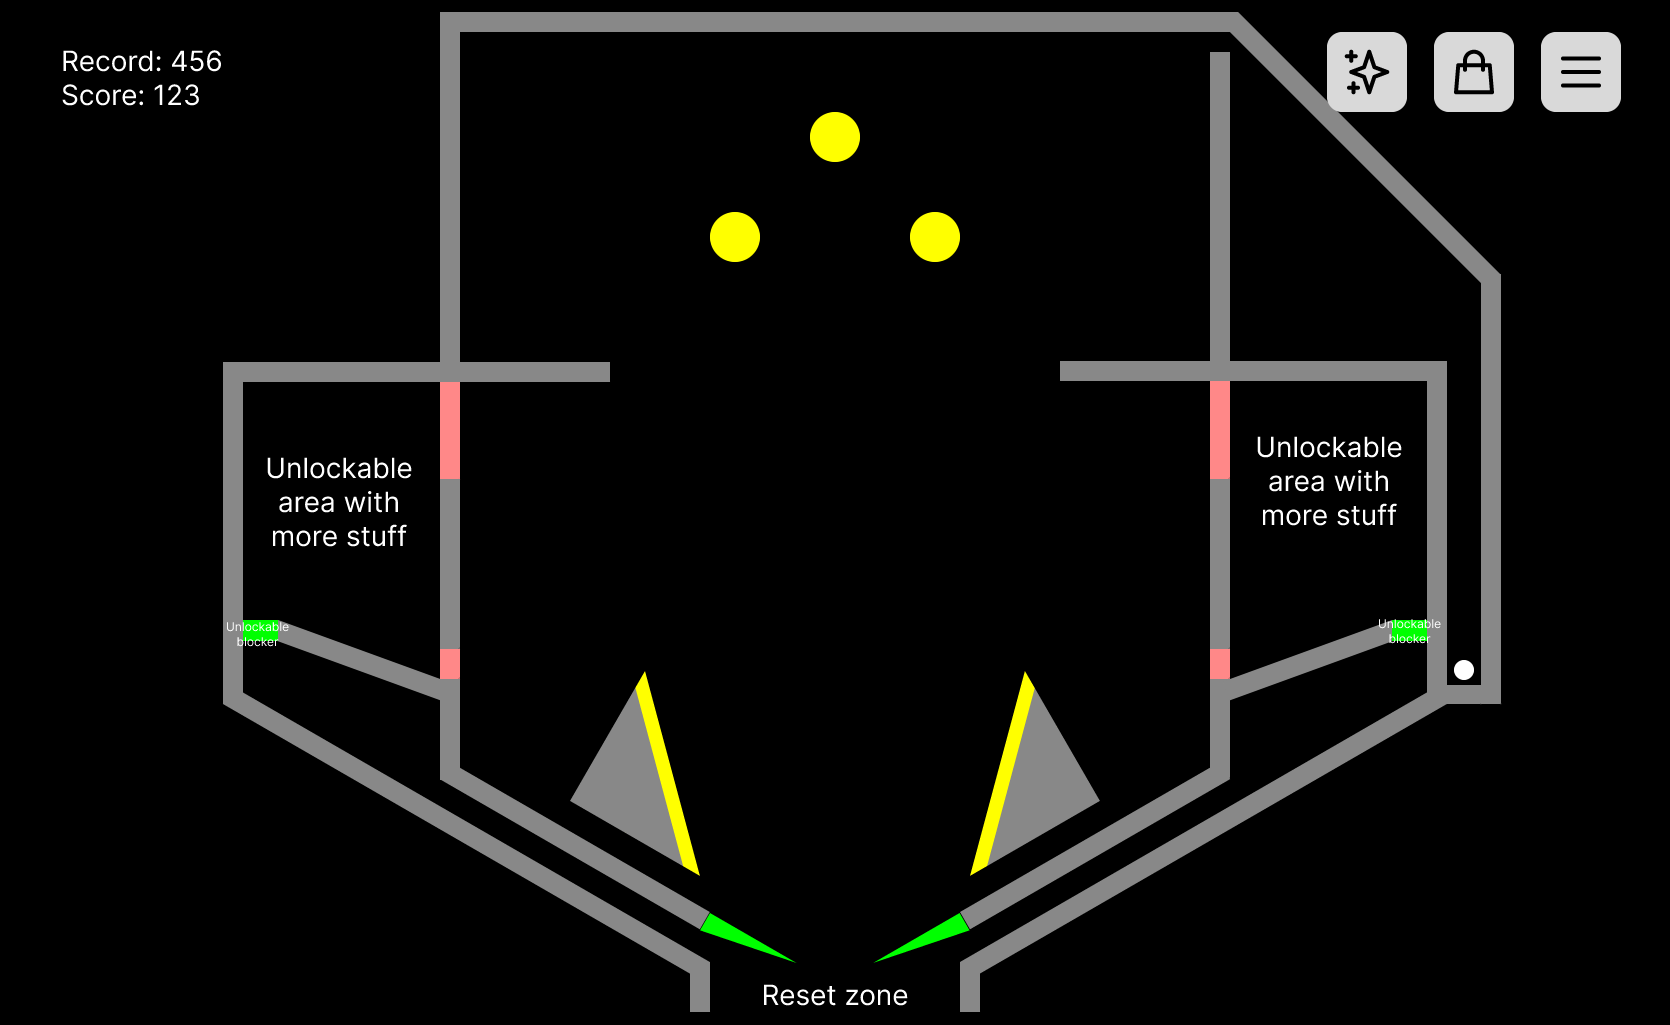
\includegraphics[width=1\linewidth]{pictures/Pinball Figma.png}
    \caption{Pinball (in Figma)}
    \label{fig:pinball}
\end{figure}
\begin{figure}[!ht]
    \centering
    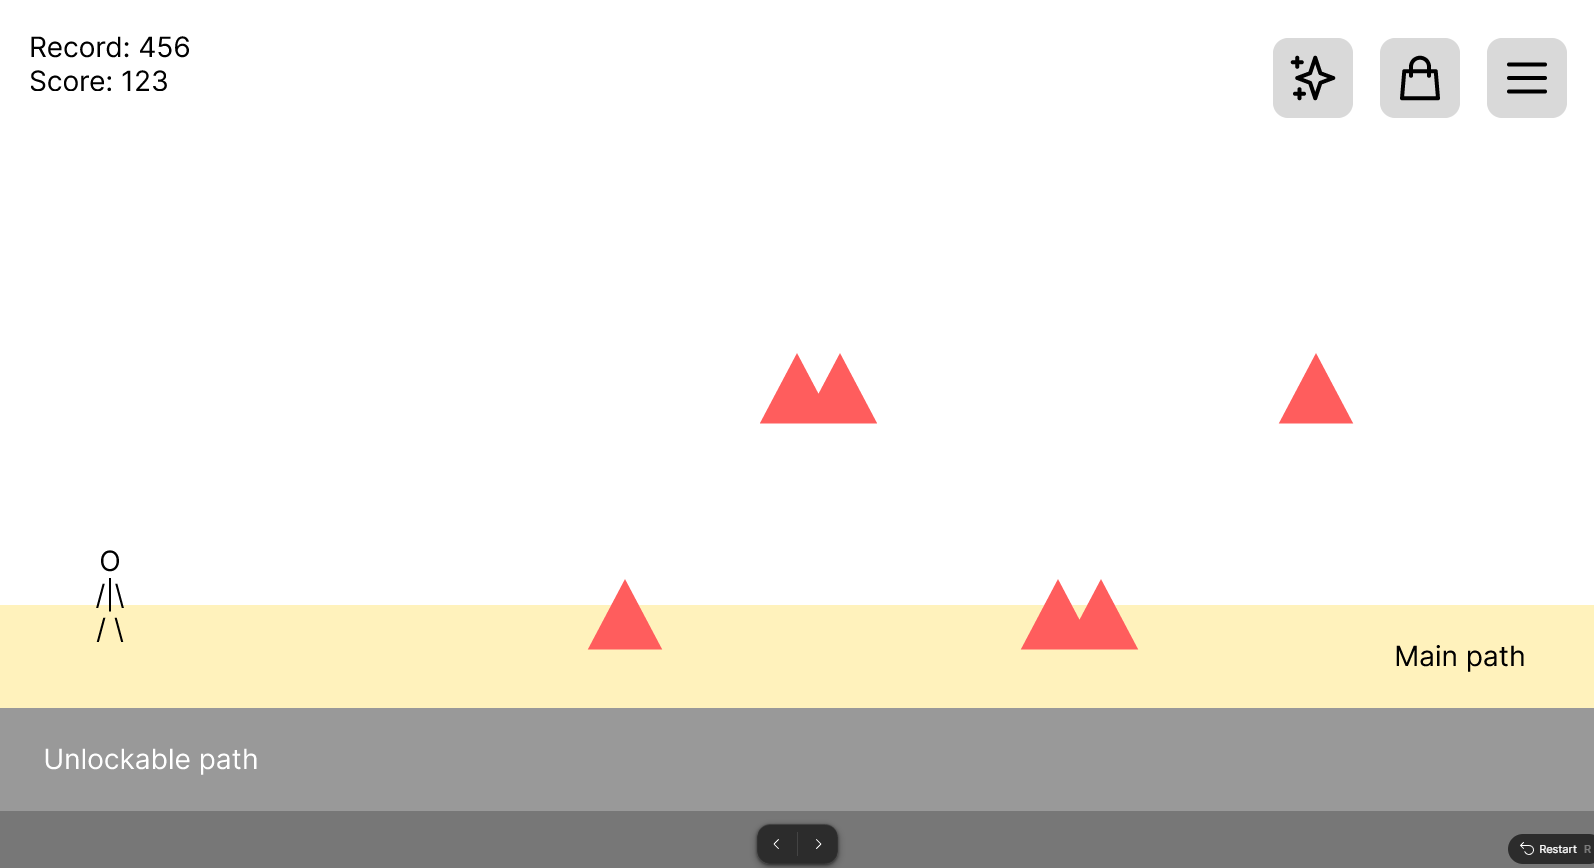
\includegraphics[width=1\linewidth]{pictures/Runner Figma.png}
    \caption{Runner (in Figma)}
    \label{fig:runnar}
\end{figure}

The mini-games will be implemented on frontend of the application, they will give data like score, achivements and earned in-game currency to the web server on backend. Backend will provide information like what extensions and modifiers should be applied to a given game. MVC style.

\subsection{How it addresses user requirements}
The creature of the application will lose energy when games are being played, but through playing, the user will be able to gain in-game currency with which they'll be able to purchase specific items at the shop to speed up the energy regeneration so they can play more games if they wish.

The user will also be able to progress to various game modifiers and extensions which should make the game more interesting as the user spends more time playing and gaining money. These modifiers should in turn provide a higher level a of challenge and reward so that the player can get even better items in the shop.

These additions should make the games have a presence outside of themselves and should address the user survey points. For example point number 3 would be solved by adding a mechanic where you can accelerate the initial easier stage of the Runner game so that the player will not get bored of playing through a difficulty level which they easily beat every time they start the game.
\newpage


 %% --------------------- JM -----------------------------------------------------------------------
\section{GUI Draft - Jaroslav Mervart}
\subsection{User survey}
The survey was primarily conducted in person among high-school and university students. My main questions were:

\begin{enumerate}
    \item Do players desire for another virtual pet game?
    \item Specification, e.g. mini-games, interaction with the in-game environment and the lack of simplicity often present in games today.
\end{enumerate}

\noindent As for summarized answers to the individual questions:

\begin{enumerate}
    \item If such game would be targeted towards audiences of all ages, not just children.
    \item[2] Audience expressed strong desire for more fleshed out mini-games, possibly recreations of older games, mostly out of nostalgia.
    \item[2] After being shown examples of virtual pet games, such as Pou~\ref{source:others/pou} or Tamaweb~\ref{source:others/tamaweb} (web-app alternative of Tamagotchi), audience did agree that clearer controls and interaction with the in-game world were in order.
    \item[2] The simplicity aspect is to be considered inconclusive, since the answer varied from person to person.
\end{enumerate}

\subsection{Alternatives research}
\subsubsection{Neopets~\ref{source:others/neopets}}
This is a very large game, and while we don't aim this high, some outstanding features can be noted.
It's advantages are:
\begin{itemize}
    \item Rich in-game environment with lots of \textbf{different} activities/mini-games is enticing to users.
    \item Nostalgia -- a lot of users came back for this reason only.
\end{itemize}
Disadvantages:
\begin{itemize}
    \item Monetization through ads.
    \item Outdated graphics.
    \item UX is criticised for being unpleasant.
\end{itemize}
\begin{figure}[H]
    \centering
    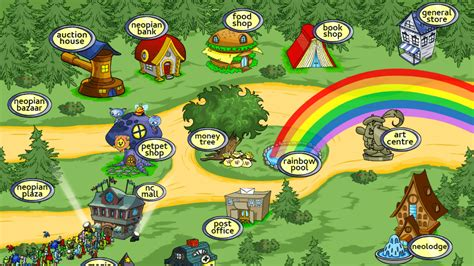
\includegraphics[width=0.5\linewidth]{pictures/neopets.jpg}
    \caption{\href{https://www.polygon.com/gaming/23824451/neopets-new-era-world-of-neopia-leadership/}{Neopets article}}
\end{figure}

\subsubsection{inQubi~\ref{source:others/inqubi}}
Offers virtual pet experience too, with a way to socialize with other players.
Advantages:
\begin{itemize}
    \item Modern GUI set in a 3D world, offers customizability.
    \item Arcade style mini-games.
    \item Progress and rewards.
\end{itemize}
Disadvantages:
\begin{itemize}
    \item Microtransactions.
    \item Small number of mini-games to play.
    \item Design might not fit everyones tastes -- \href{https://en.wikipedia.org/wiki/Uncanny_valley}{uncanny valley}.
\end{itemize}

\begin{figure}[H]
    \centering
    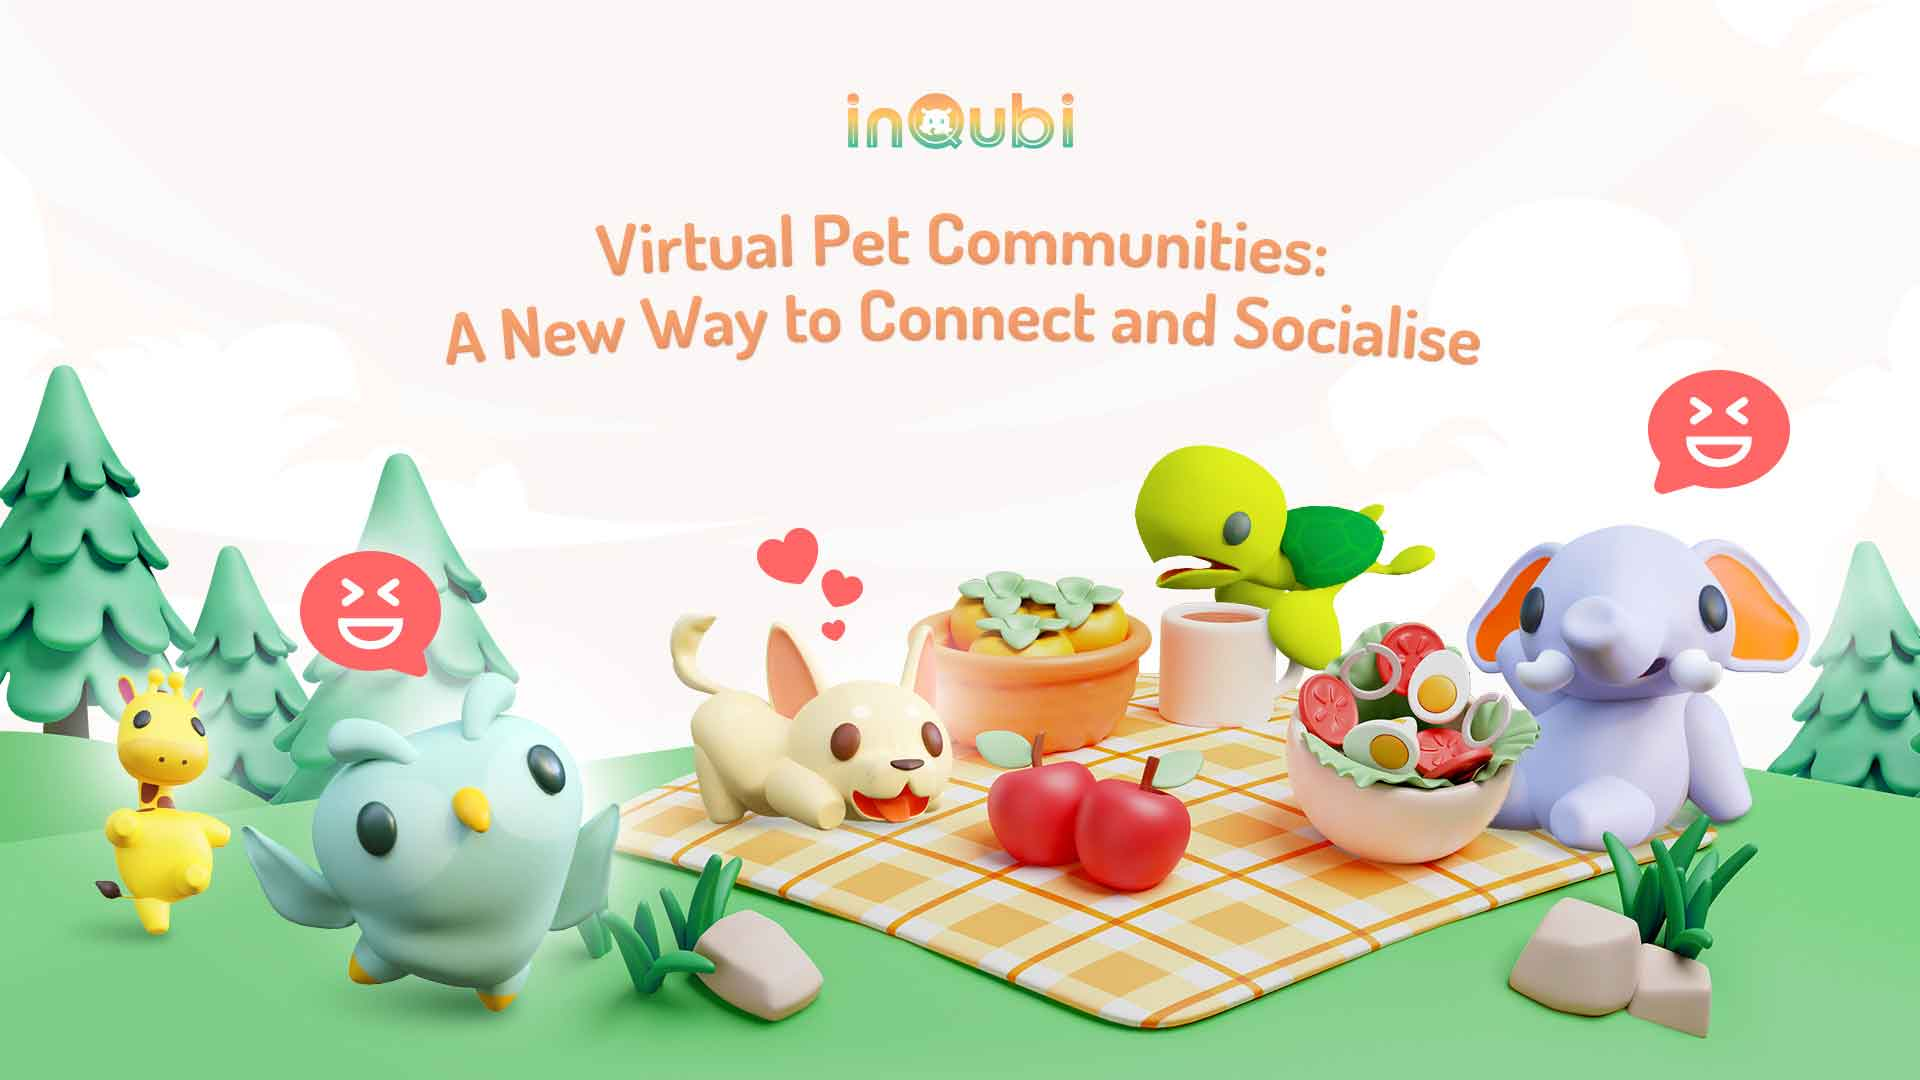
\includegraphics[width=0.5\linewidth]{pictures/inqubi.jpg}
    \caption{\href{https://inqubi.com/blog/virtual-pet-communities-connect-socialise/}{inQubi blog}}
\end{figure}

\subsubsection{Solitaire~\ref{source:others/solitaire}}
As original Microsoft games are nostalgic for the very reason of being shipped with every older version of Windows, I took a look into the design of original Microsoft Solitaire~\ref{source:others/solitaire}. Going with a simple design seems to be the preferred approach
\begin{figure}[!ht]
    \centering
    \includegraphics[width=0.5\linewidth]{pictures/Solitaire.png}
    \caption{Microsoft Solitaire~\ref{source:others/solitaire}}
\end{figure}

\subsection{Description of the proposed GUI}

My proposal consists of two independent components. 
The first is an alternative to the classic Microsoft \textbf{Solitaire}~\ref{source:others/solitaire}, serving as a mini-game. 

The second is a \textbf{scrollable achievement menu} which, while still simple, will be heavily dependent on the data it receives in order to display \emph{(un)locked} achievements correctly. 
Therefore, not only must the achievements menu be implemented, but also the \textit{triggers} (event-based conditions) and \textit{progression counters} for the achievements themselves throughout the application.

As for Solitaire itself, it must correctly display the states of the cards, allow or block moves, and automatically save the session.

The simple appearance of both components may change in the future.

\begin{figure}[H]
    \centering
    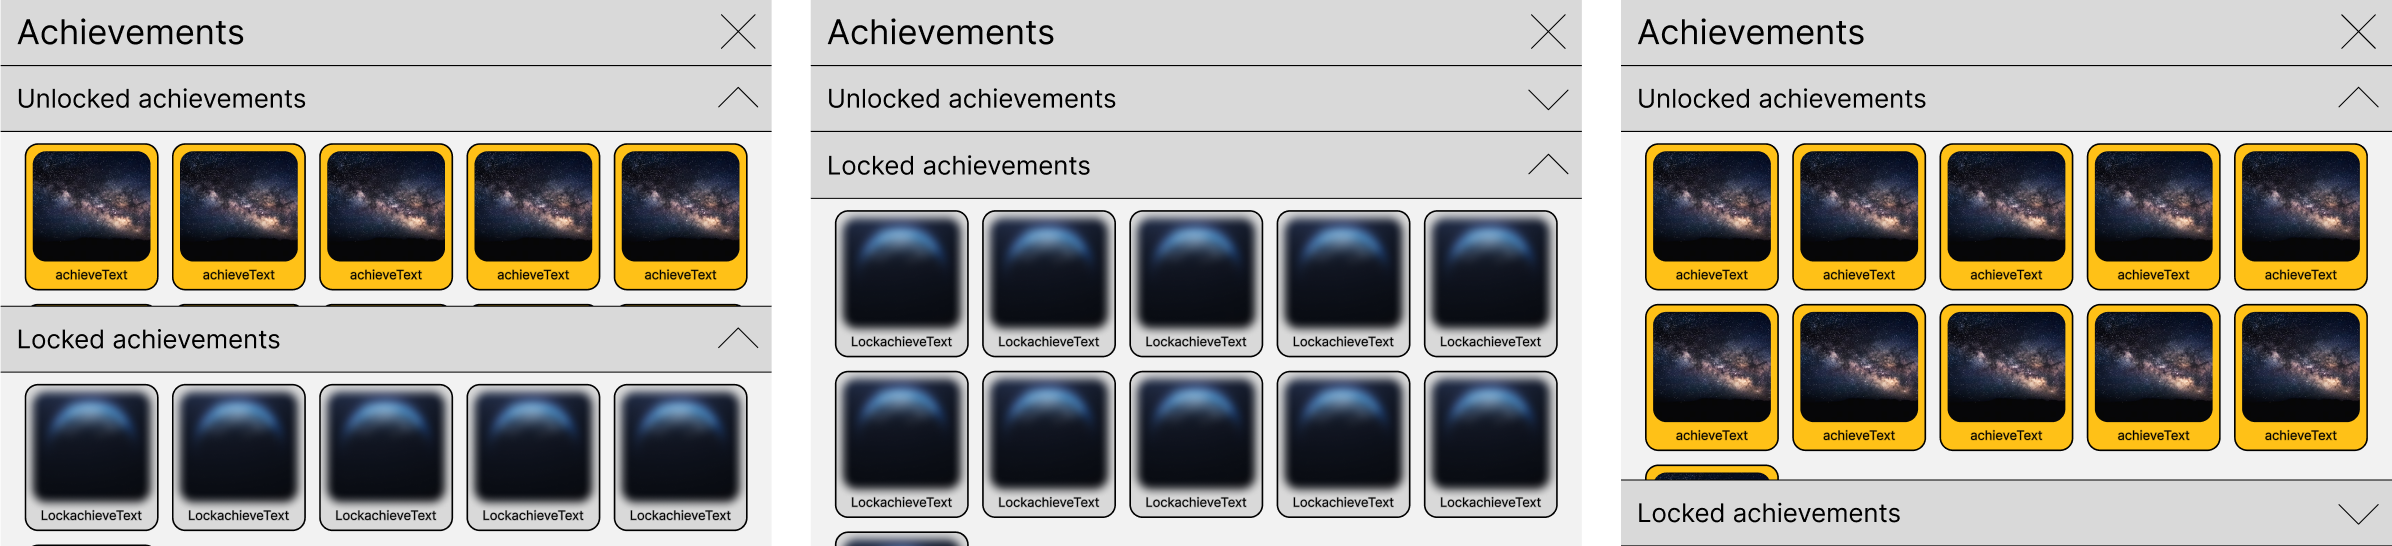
\includegraphics[width=1\linewidth]{pictures/achievements.png}
    \caption{Achievements menu}
    \label{fig:achievements}
\end{figure}
\begin{figure}[H]
    \centering
    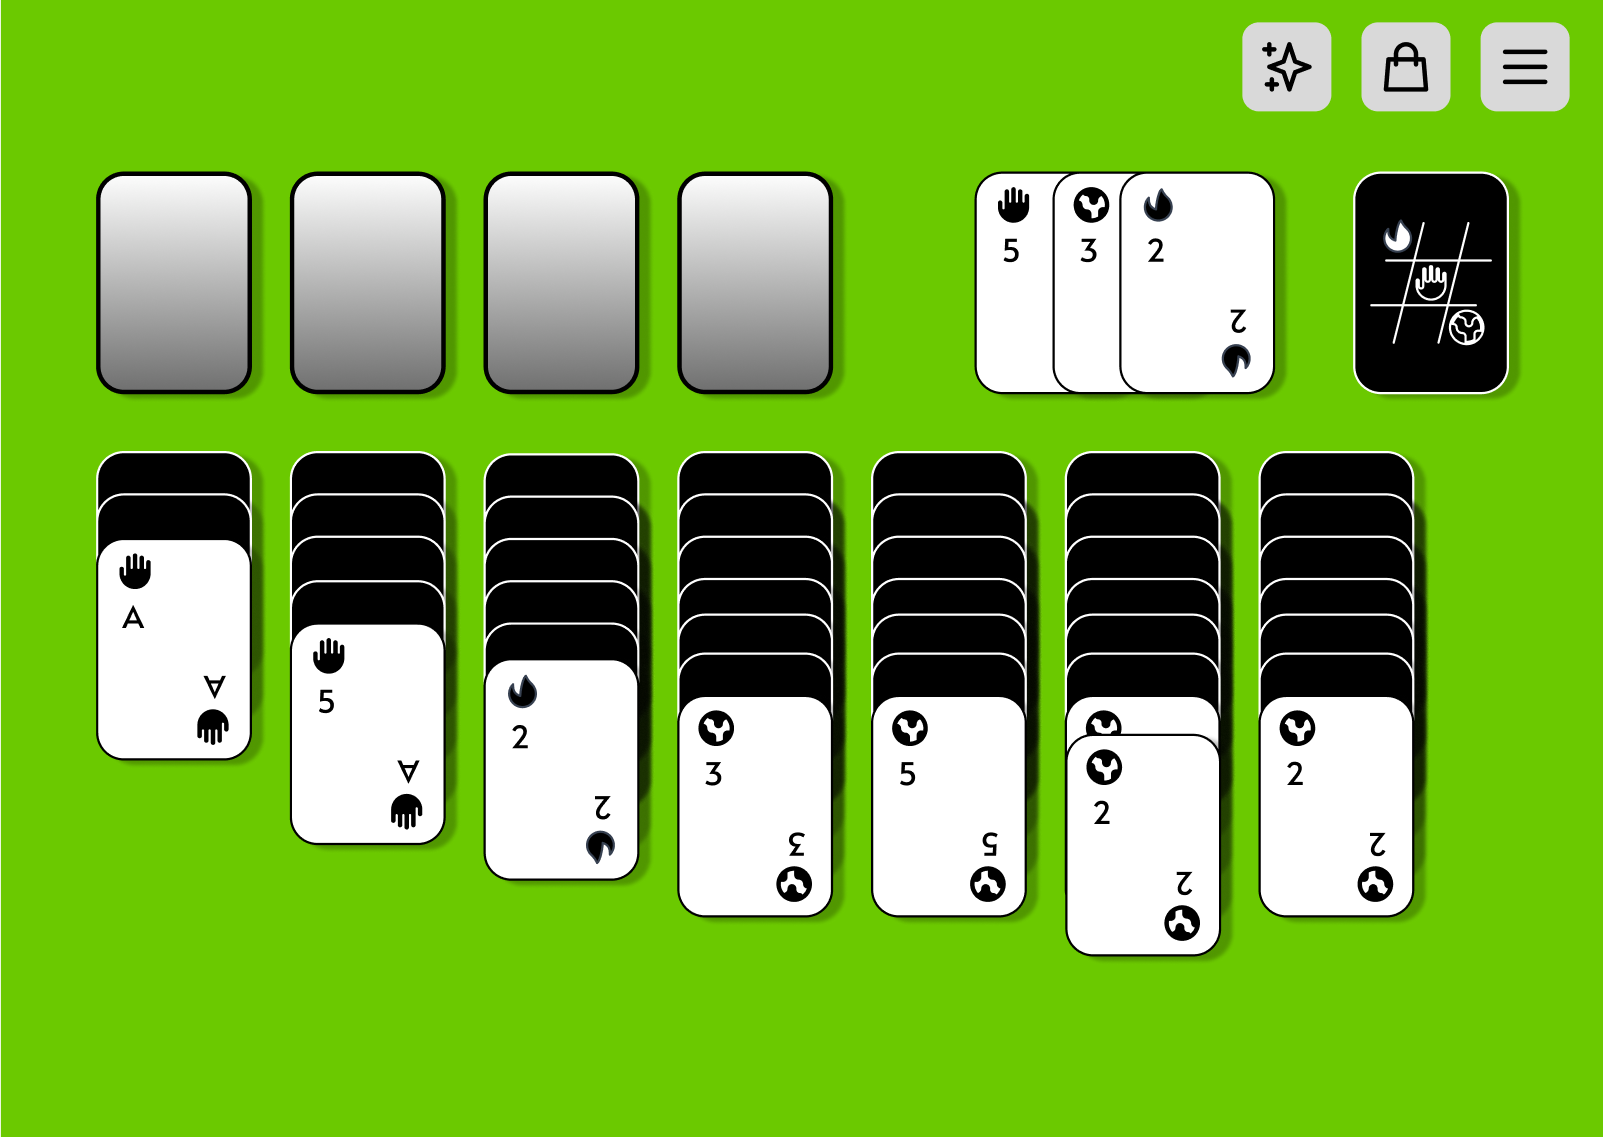
\includegraphics[width=0.4\linewidth]{pictures/solitaire.png}
    \caption{Solitaire mini-game}
    \label{fig:solitaire_game}
\end{figure}

\subsection{How it addresses/reflects user requirements}

My draft offers simple yet nostalgic elements mixed with an achievement system applicable not only to my mini-game but also throughout the application, giving the user a sense of progression. 
The Solitaire game is straightforward to play, well suited for desktop resolutions, and doesn't require the user to stress about exiting or saving the game. 
This game could reward the user with a certain amount of coins based on the time they have managed to finish the game, keeping the system simple and fair. 
A randomizer (which will follow specific rules in order to make the game playable) will also need to be implemented. 

The frontend itself will draw the structure from the server, informing the server when a user attempts to make a move and updating the local game state accordingly. 
\newpage
 %% --------------------- JM -----------------------------------------------------------------------

%% --------------------- USED TECH-----------------------------------------------------------------
\section{Used Technologies}
\subsection{Frontend FE}
For creation of our GUI we have chosen React with the tool Vite. We have chosen React because it allows us to make an interactive componented GUI which can be expanded quite easily. Vite provides us a fast development server with an instant hot reload. We are using Axios for calling our backend, it provides a simple interface for working with REST API. For basic stylisation we use CSS.
\subsection{Backend BE}
For creation of our backend we have chosen Python language with the framework Flask. Flask is a simple and easily configurable framework which allows us to quickly create REST API. The application logic is divided into separate modules, like \texttt{creature\_state.py}, \texttt{server.py} and mini-games in their separate files. Flask also supports the MVC design pattern. Communication between FE and BE works by HTTP REST API with JSON data. For simulating game states and managing user inputs we are using internal modules in Python.

\subsection{Summarty of used libraries and tools}
\begin{itemize}
    \item Vite - Build and dev server for React
    \item React - GUI with components
    \item Axios - HTTP client
    \item Matter.js - 2D physics
    \item Flask (Python) - logic and model
    \item Python standard libs - score and state saving
\end{itemize}

 %% --------------------- BE API-------------------------------------------------------------------
\section{Backend API Draft}
\subsection{Separation of FE, BE and app-logic}
\textbf{Application Architecture}

[React (Vite) FE]
\begin{itemize}
    \item axios $\rightarrow$ REST /api/v1
\end{itemize}

[Flask BE]
\begin{itemize}
    \item Controllers (endpoints)
    \item Services (game logic, cooking recipes, creature status, scoring)
    \item Models (data classes / ORM)
    \item Storage (in-memory, database)
\end{itemize}


\noindent\textbf{MVC/equivalent}
\begin{itemize}
    \item Controller = Flask route
    \item Model (state data structures)
    \item Service (application logic)
\end{itemize}

\noindent\textbf{Basic data models (only showcase, not all are present)}
\begin{table}[H]
\centering
\begin{tabular}{|l|l|l|}
\hline
\textbf{Creature state} & \textbf{GameSession} & \textbf{Recipe} \\ \hline
hunger       & id          & id          \\ \hline
clean        & game        & name        \\ \hline
energy       & state       & ingredients \\ \hline
updatedAt    & createdAt   & steps       \\ \hline
--           & finished    & durationSec \\ \hline
\end{tabular}
\end{table}

\subsubsection*{Endpoints}
\verb|GET /api/v1/health| \\
\verb|GET /api/v1/creature/feed (clean/sleep/...)| \\
\verb|POST /api/v1/pinball/score| \\
\verb|GET /api/v1/pinball/leaderboard?limit=10| \\
\verb|GET /api/v1/cooking/recipes/{id}| \\
\verb|POST /api/v1/cooking/session| \\
\verb|POST /api/v1/cooking/session/{id}/action| \\
\verb|POST /api/v1/cooking/session/{id}/finish| \\
\verb|POST /api/v1/solitaire/session| \\
\verb|POST /api/v1/dino/score| \\
\verb|GET /api/v1/dino/leaderboard?limit=10| \\
\verb|GET /api/v1/leaderboard?game=pinball&limit=10| \\

\subsubsection*{Application startup (for now)}

Backend:

\verb|python server.py|

\noindent Frontend:

\verb|npm run dev|

\newpage
%% NA screenshots keby bolo potreba stranku nasirku

%% \begin{landscape}
%%%% OBSAH
%% \end{landscape}

\section{Sources}

\subsection{Frontend}
\begin{itemize}
    \item\href{https://nodejs.org/}{\texttt{Node.js}}
    \item\href{https://react.dev/}{\texttt{React}}
\end{itemize}

\subsection{Backend}
\begin{itemize}
    \item \href{https://flask.palletsprojects.com/en/stable/}{\texttt{Python/Flask}}
\end{itemize}

\subsection{Others}
\begin{enumerate}
    \item \label{source:others/pou} \href{https://www.pou.me/}{Pou}
    \item \label{source:others/finch} \href{https://finchcare.com/}{Finch}
    \item \label{source:others/talking_tom} \href{https://talkingtomandfriends.com/}{Talking Tom}

    \item \label{source:others/tamagotchi} \href{https://en.wikipedia.org/wiki/Tamagotchi}{Tamagotchi}
    \item \label{source:others/tamaweb} \href{https://autosam.github.io/Tamaweb/}{Tamaweb}
    \item \label{source:others/zelda} \href{https://en.wikipedia.org/wiki/The_Legend_of_Zelda:_Breath_of_the_Wild}{The Legend of Zelda: Breath of the Wild}
    
    \item \label{source:others/pinball} \href{https://en.wikipedia.org/wiki/Full_Tilt!_Pinball}{Full Tilt! Pinball}
    \item \label{source:others/dinogame} \href{https://en.wikipedia.org/wiki/Dinosaur_Game}{Dinosaur Game}

    
    \item \label{source:others/neopets} \href{https://portal.neopets.com/about-neopets}{Neopets}
    \item \label{source:others/inqubi} \href{https://inqubi.com/about/}{inQuibi}
    \item \label{source:others/solitaire} \href{https://en.wikipedia.org/wiki/Microsoft_Solitaire}{Microsoft Solitaire}
    
\end{enumerate}
\end{document}
